This section shows a real example of how to combine three of the \abcpt{}s created: \catabc{},
\pasteabc{} and \learningabc{}.

In this example, a user wants to study his voice (\emph{Tenor}) and \emph{Soprano}'s on the first three sections
of the \emph{Christmas Villancico}\footnote{A Villancico is a musical and poetic form written in
Spanish and Portuguese, traditional from Spain, Latin America and Portugal. These pieces were
popular between century XV and XVIII.} \textit{Verbum caro factum est}.

Each section and voice is written in separate files, so the parts requested will be assembled by
combining \pasteabc{} with \catabc{}.

Then \learningabc{} is going to be used with the combined score in order to produce two scores: one
where voice \emph{Tenor} is highlighted and another where the other voices are.

Listing \ref{lst:cat_paste_by_example} shows the first step being put into action. Listing
\ref{lst:verbum} shows its output, which, in this section, is going to be referred to as
\emph{verbum.abc} and figure \ref{fig:verbum} the corresponding score.\\

\begin{lstlisting}[caption={\catabc{} and \pasteabc{} by example},label={lst:cat_paste_by_example},captionpos=t,abovecaptionskip=-\medskipamount]
cat_abc (
  paste_abc ( 101.abc 103.abc )
  cat_abc   ( 201.abc 303.abc )
) > verbum.abc
\end{lstlisting}

\vspace{1cm}
\lstinputlisting[caption={\emph{verbum.abc}},label={lst:verbum},captionpos=t,abovecaptionskip=-\medskipamount]{misc/verbum.tex}

% \vspace{-1.30cm}
\begin{figure}[H]
  \centering
  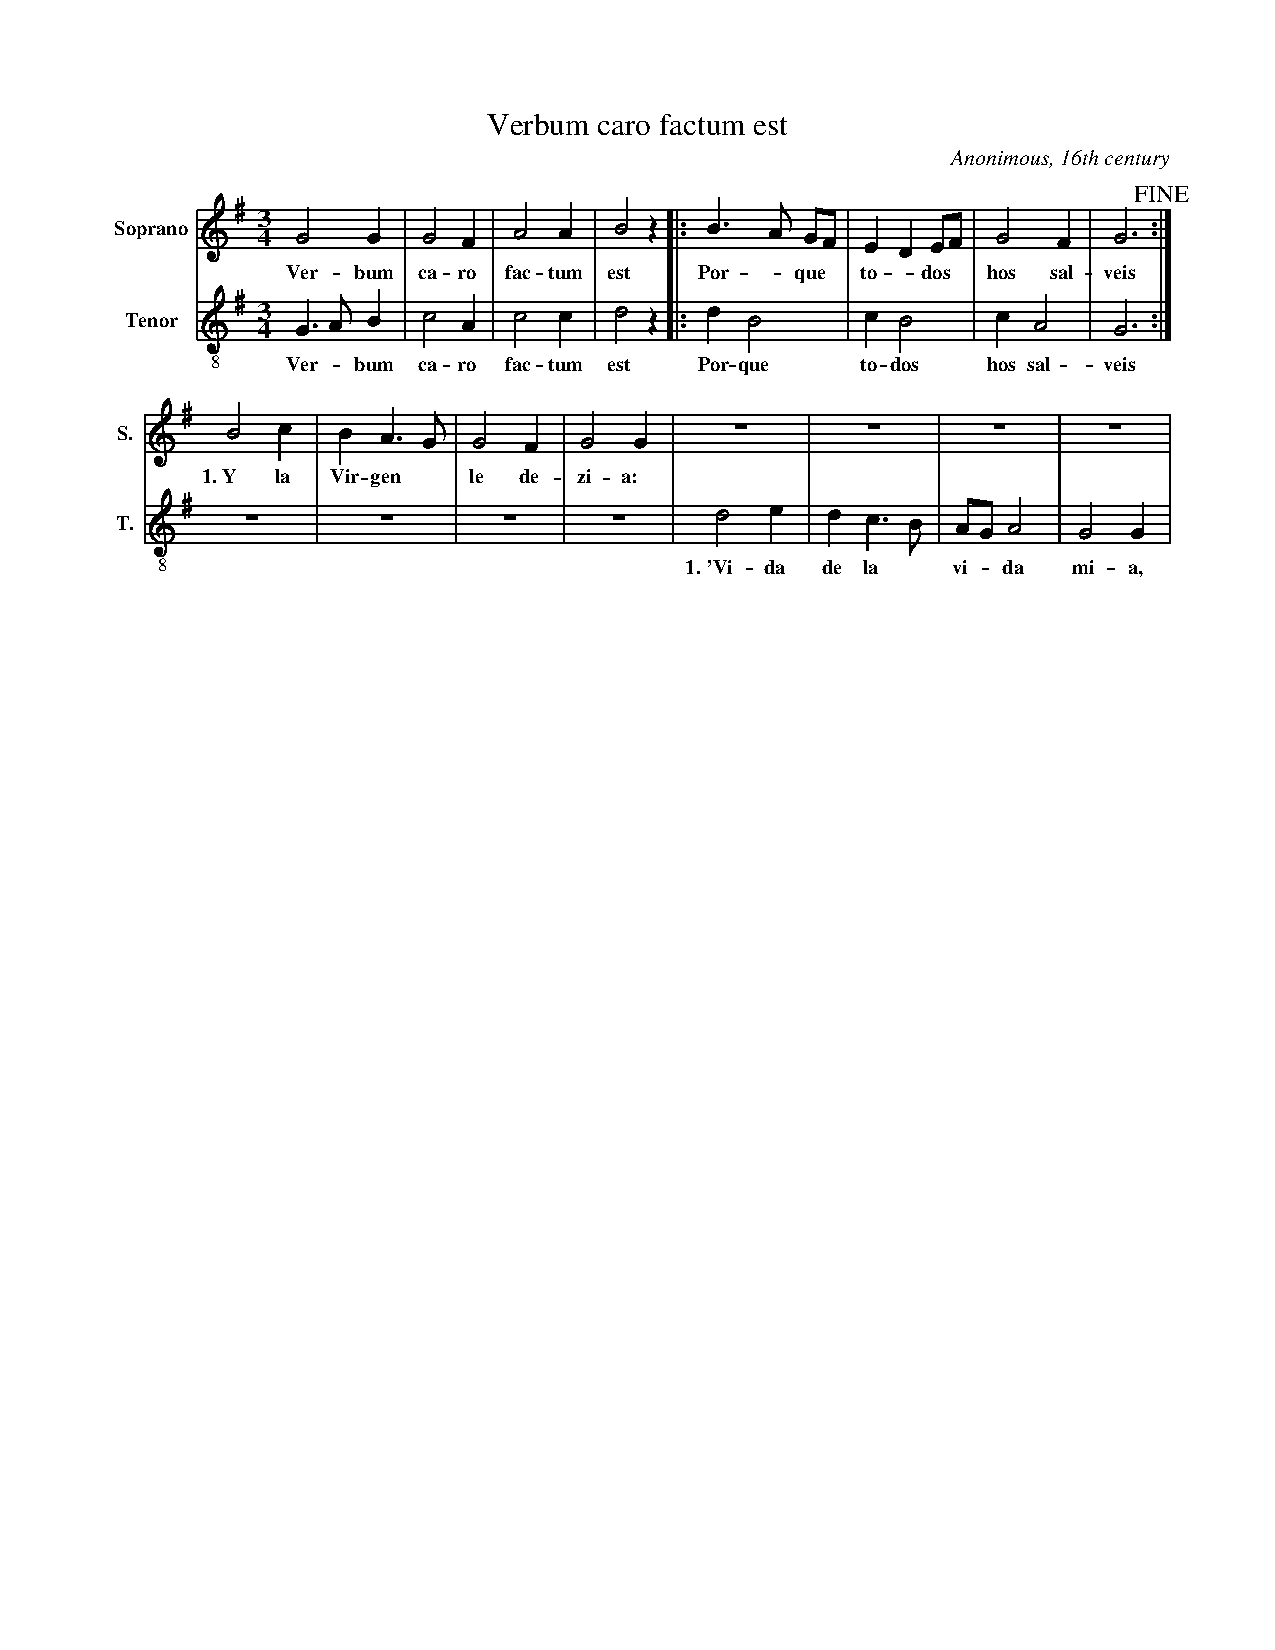
\includegraphics[width=0.8\textwidth, clip=true, trim = 15mm 180mm 15mm 30mm]{img/verbum.pdf}
  \caption{Verbum caro factum est Score: Sections 1, 2 \& 3; Parts 1 \& 3}
  \label{fig:verbum}
\end{figure}

After putting the score together, it's time to modify it in order to help the user study. So
\learningabc{} (see listing \ref{lst:learning_on_cat_paste}) generates a score where just voice
\emph{Tenor} is highlighted (\ref{lst:just_tenor}) and one where all voices but \emph{Tenor}'s are
highlighted (\ref{lst:all_but_tenor}).\\

\begin{lstlisting}[caption={\learningabc{} on combined score},label={lst:learning_on_cat_paste},captionpos=t,abovecaptionskip=-\medskipamount]
learning_abc -v=Tenor verbum.abc
\end{lstlisting}

\lstinputlisting[caption={verbum\_just\_Tenor.abc},label={lst:just_tenor},captionpos=t,abovecaptionskip=-\medskipamount]{misc/v_just_Tenor.tex}
\lstinputlisting[caption={verbum\_all\_but\_Tenor.abc},label={lst:all_but_tenor},captionpos=t,abovecaptionskip=-\medskipamount]{misc/v_all_but_Tenor.tex}
